\documentclass[twocolumn]{revtex4}
\usepackage[]{graphicx}


\begin{document}
\title{Journal Article - Human v Velociraptor}
\author{Torri Halaquist}
\affiliation{Siena College, Loudonville, NY}
\date{\ December 15, 2015}
\begin{abstract}
    Throughout the course of this project, the question of whether of not a human can outrun the predator of the velociraptor. After completion, there will be four questions answered as well as two graphs in support of the result determined. With an understanding of physics and the the plotting capability of Python, the problem can be solved. Using the velocity equation of (v=d/t) and probability equations, the chances of the velociraptor catching up to the human can be calculated, and the point at which the 'raptor reaches the human is visually shown on the graphs. By solving the questions, the results show that even though the velociraptor reaches the human quickly, the chance that it is successful in attempting to bite the human are 20 percent, 15 percent, and 7 percent with the first, second, and third tries, respectively. The probability that the human escapes are proven to vary between 58-63 percent success as proven with repeated trials. Therefore, even though the human cannot outrun the velociraptor, the person is still likely to survive the chase. 
\end{abstract}

\maketitle

\section{Introduction}
The completion of the project was carried out using different strategies of the capabilities of Python, but the most important idea to focus on is keeping track of all of the variables used in the problems. Below are explanations of how each problem was solved, graphs included for the Questions 1 and 3.

\section{Question 1}
\subsection{Make a plot of the position vs time for the human and the 'raptor.}
This problem includes the given information of the human speed being equal to 3 meters per second with a 30 meter head start and the velociraptor speed equal to 18 meters per second. Using this, a graph of position vs time can be produced for both the human and the 'raptor. Because time is a constant variable for both of the beings in question, a empty list is made representing all of the times within a factor of 0.001 to determine when the 'raptor catches the person using the for loop "for i in range(0,500) and appending the resulting times into the previously empty time list. In terms of distance traveled when caught, both use a similar equation, multiplying the speed by the list of times. The only difference is that the human's data includes an addition of the 30 meter head start to the equation. Using the graph functions incorporated in Python, the data of the human position v time and velociraptor position v time can be plotted on the same graph and compared.


\begin{figure}[h]
\centering
\footnote{This graph includes both the human data in blue and the velociraptor data in green.\label{fig:graph1}}
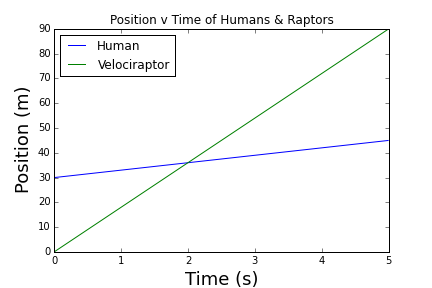
\includegraphics[width=0.5\textwidth]{final_graph_1.png}
\end{figure}

\section{Question 2}
\subsection{How far has the human traveled/How much time has passed when the 'raptor catches up?}
One of the benefits of solving this question is that the graph from question 1 shows what the catch-up time and distance are, and because of this, self-check is provided right into the project. When all of the coding is done for this question, the results that print to the screen should prove what the graph visually displays.To start, the function catch-up was defined to intake human position, 'raptor position-r, and time, t. Again using a range from 0-500, 500 positions were analyzed between the starting point and the meeting point to determine the distance traveled. In this question, an "if" statement was used to return the time passed and human position traveled if the raptor position equals the human position (confirming they caught up to each other). The code then printed the numerical value of time and distance to be 2 seconds and 36 meters, respectively.
\subsection{Algebraic Equation}
The algebraic equation used to determine the distance that Python used code to determine is:
$$d=\frac{\frac{30m}{v_r}}{{\frac{1}{v_h}}-{\frac{1}{v_r}}}$$
these equations are used to solve for the value of d. Once a value for the distance is solved for, either of the following equations can be used to solve for time:
$$ t = \frac{d+30m}{v_r} $$ $$t = \frac{d}{v_h} $$

The variables for these equations represent:
($d$) = distance human travels until caught
($d+30m$) = distance 'raptor travels to catch human (including human head start)
($v_h$) = speed of human
($v_r$) = speed of raptor
($t$) = time

\section{Question 3}
\subsection{If the 'raptor can begin to attack from one meter away, how much time has passed and how far has human traveled?}
In this question, the same graph is pulled from question 1, although there is an additional arrow plotted on the graph to represent where the 'raptor begins to attempt to bite the human, while still one meter away from completely catching up to the person. To determine the location of which the arrow needs to point, a new equation needs to defined that takes the gap of one meter into consideration in comparison to the equation from question one. Therefore, the first step is define an equation attempted-bite that takes human position, raptor position-r, and time t in. Then using a for loop of for i in range(0,500), 500 positions are considered between starting point and one meter gap. Using an "if" statement to determine the location when the gap between the human and the raptor is one meter   (position[i]-position-r[i] < 1), the code will return the time and position of this location, and then printing the human distance traveled and time passed by the statements included in the code.
\subsection{Algebraic Equation}
The algebraic equation used to determine the distance that Python used code to determine is:
$$d=\frac{\frac{29m}{v_r}}{{\frac{1}{v_h}}-{\frac{1}{v_r}}}$$
these equations are used to solve for the value of d. Once a value for the distance is solved for, use either of the following equations to solve for time:
$$ t = \frac{d+29m}{v_r} $$ $$t = \frac{d}{v_h} $$
The variables still represent the same values, only d+29m represents the distance the 'raptor travels to catch the human because of the human headstart minus the one meter gap.
\begin{figure}[h]
\centering
    \includegraphics[width=0.5\textwidth]{final_graph_2.png}
\footnote{This graph includes both the human data in blue and the velociraptor data in green.\label{fig:final_graph_2.png}}
\end{figure}

\section{Question 4}
\subsection{What is the probability the human will escape the bite of the velociraptor?}
In the background of this question, the data of the velociraptors probability for succesfful biting are 20 percent on the first try, 15 percent on the second, and then only 7 percent on the third. After the third try if the 'raptor has been unsuccessful all three times, the human will have been able to escape and is safe. To start the problem, the function survive is defined. Three separate equations were created under this equation, using random data to determine the number of times that the 'raptor will successfully bite the human the first, second, and third tries. A series of if, elif, and else statements in regards to being less than or equal to the mentioned percentages are used in order to determine the number of times the 'raptor got the human, returning 'bit' or returning 'missed' if the person got away. For example, if attempt1 is less than or  equal to 20: return "Bit," where the code will then stop if the 'raptor was successful or move on to attempt2 if it was not. Next, empty lists. The code runs through each of these equations and if is unsuccessful in biting the human after the third try, it returns "missed" and the human is safe. Then, variables "deaths" and "escapes" are defined with a starting value of zero. Using a for loop for i in range(0,1000), one thousand cases are tested to determine an accurate probability of escape. The code then runs through the one thousand trials one at a time (by order of i+=1) and if the trial returns "bit," one trial is added to the "deaths" variable (deaths += 1), or the "escapes" variable if "missed" is returned (escapes +=1). With the data recorded in the variables, the percent chance of outrunning the raptor is calculated by dividing the number of escapes by 1000 trials, then multiplying by 100 to represent a percentage. Because random data is used, the probability varies between 58-63 percent of escaping the 'raptor.

\section{In Closing}
Through the use of the formulas, strategies, and plotted graphs included in this document, the question of the probability of a human being able to escape a velociraptor was proven to vary between 58 and 63 percent. By using the graphs Python code, and the algebraic equations, the answers self-check and ensure accuracy. By incorporating both of these tactics, the project could be completed correctly and determine that majority of the time, a human could in fact escape a velociraptor.
\end{document}
